% -*- latex -*-

\chapter{Control Environment}
\label{chap:ControlEnvironment}

\index{control~environment|(}
\index{environment!control|(}

The control environment is where code interfaces with applications and I/O
devices. The associated API is designed for users that want to use VTK-m to
analyze their data using provided or supplied worklets. Code for the
control environment is designed to run on a single thread (or one single
thread per process in an MPI job).

Most users of VTK-m will have some interaction with the control
environment, for you cannot define data structures or execute any
algorithms without it.

\section{Dynamic Array Handle}
\label{sec:DynamicArrayHandle}

\index{dynamic~array~handle|(}
\index{array~handle!dynamic|(}

The \textidentifier{ArrayHandle} class uses templating to make very
efficient and type-safe access to data. However, it is sometimes
inconvenient or impossible to specify the element type and storage at
run-time. The \textidentifier{DynamicArrayHandle} class provides a mechanism
to manage arrays of data with unspecified types.

\vtkmcont{DynamicArrayHandle} holds a reference to an array. Unlike
\textidentifier{ArrayHandle}, \textidentifier{DynamicArrayHandle} is
\emph{not} templated. Instead, it uses C++ run-type type information to
store the array without type and cast it when appropriate.

\index{dynamic~array~handle!construct}
A \textidentifier{DynamicArrayHandle} can be established by constructing it
with or assigning it to an \textidentifier{ArrayHandle}. The following
example demonstrates how a \textidentifier{DynamicArrayHandle} might be
used to load an array whose type is not known until run-time.

\vtkmlisting{Creating a \textidentifier{DynamicArrayHandle}.}{CreateDynamicArrayHandle.cxx}

\subsection{Querying and Casting}
\label{sec:DynamicArrayHandleQueryingAndCasting}

\index{dynamic~array~handle!query}
Data pointed to by a \textidentifier{DynamicArrayHandle} is not directly
accessible. However, there are a few generic queries you can make without
directly knowing the data type. The \textcode{GetNumberOfValues} method
returns the length of the array with respect to its base data type. It is
also common in VTK-m to use data types, such as \vtkm{Vec}, with multiple
components per value. The \textcode{GetNumberOfComponents} method returns
the number of components in a vector-like type (or 1 for scalars).

\vtkmlisting{Non type-specific queries on \textidentifier{DynamicArrayHandle}.}{NonTypeQueriesDynamicArrayHandle.cxx}

\index{dynamic~array~handle!new~instance}
It is also often desirable to create a new array based on the underlying
type of a \textidentifier{DynamicArrayHandle}. For example, when executing
a worklet \fix{or filter?} on one or more fields, it is common to generate
an output field, and it is furthermore usually desirable for the output
type to match the input type. To satisfy this use case,
\textidentifier{DynamicArrayHandle} has a method named
\textcode{NewInstance} that creates a new empty array with the same
underlying type as the original array.

\vtkmlisting{Using \textidentifier{DynamicArrayHandle}\textcode{::NewInstance()}.}{DynamicArrayHandleNewInstance.cxx}

Before the data with a \textidentifier{DynamicArrayHandle} can be accessed,
the type and storage of the array must be established. This is usually done
internally within VTK-m when a worklet \fix{or filter?} is invoked.
However, it is also possible to query the types and cast to a concrete
\textidentifier{ArrayHandle}.

\index{dynamic~array~handle!query}
You can query the component type and storage type using the
\textcode{IsArrayHandleType}, \textcode{IsSameType}, and
\textcode{IsTypeAndStorage} methods. \textcode{IsArrayHandleType} takes an
example array handle type and returns whether the underlying array matches
the given static array type. \textcode{IsSameType} behaves the same as
\textcode{IsArrayHandleType} but accepts an instances of an
\textidentifier{ArrayHandle} object to automatically resolve the template
parameters. \textcode{IsTypeAndStorage} takes an example
component type and an example storage type as arguments and returns whether
the underlying array matches both types.

\vtkmlisting{Querying the component and storage types of a \textidentifier{DynamicArrayHandle}.}{QueryDynamicArrayHandle.cxx}

\index{dynamic~array~handle!cast}
Once the type of the \textidentifier{DynamicArrayHandle} is known, it can
be cast to a concrete \textidentifier{ArrayHandle}, which has access to the
data as described in Section~\ref{sec:ArrayHandle}. The easiest way to do
this is to use the \textcode{CopyTo} method. This templated method takes a
reference to an \textidentifier{ArrayHandle} as an argument and sets that
array handle to point to the array in \textidentifier{DynamicArrayHandle}.
If the given types are incorrect, then \textcode{CastToArrayHandle} throws
a \vtkmcont{ErrorControlBadValue} exception.

\vtkmlisting{Casting a \textidentifier{DynamicArrayHandle} to a concrete \textidentifier{ArrayHandle}.}{CastDynamicArrayHandle.cxx}

\subsection{Casting to Unknown Types}

\index{dynamic~array~handle!cast|(}

Using \textcode{CastToArrayHandle} is fine as long as the correct types are
known, but often times they are not. For this use case
\textidentifier{DynamicArrayHandle} has a method named
\textcode{CastAndCall} that attempts to cast the array to some set of
types.

The \textcode{CastAndCall} method accepts a functor to run on the
appropriately cast array. The functor must have an overloaded const
parentheses operator that accepts an \textidentifier{ArrayHandle} of the
appropriate type.

\vtkmlisting[ex:UsingCastAndCall]{Operating on \textidentifier{DynamicArrayHandle} with \textcode{CastAndCall}.}{UsingCastAndCall.cxx}

\subsection{Specifying Cast Lists}
\label{sec:DynamicArrayHandleSpecifyingCastLists}

The \textcode{CastAndCall} method can only check a finite number of types.
The default form of \textcode{CastAndCall} uses a default set of common
types. These default lists can be overridden using the VTK-m list tags
facility, which is discussed at length in Section~\ref{sec:ListTags}. There
are separate lists for component types and for storage types.

Common type lists for components are defined in
\vtkmheader{vtkm}{TypeListTag.h} and are documented in
Section~\ref{sec:TypeLists}. This header also defines
\vtkmmacro{VTKM\_DEFAULT\_TYPE\_LIST\_TAG}, which defines the default list
of component types tried in \textcode{CastAndCall}.

\index{tag!storage lists|(}
\index{lists!storage|(}
\index{storage lists|(}

Common storage lists are defined in
\vtkmheader{vtkm/cont}{StorageListTag.h}. There is only one common storage
distributed with VTK-m: \textidentifier{StorageBasic}. A list tag
containing this type is defined as \vtkmcont{StorageListTagBasic}.

As with other lists, it is possible to create new storage type lists
using the existing type lists and the list bases from
Section~\ref{sec:BuildingListTags}.

The \vtkmheader{vtkm/cont}{StorageListTag.h} header also defines a macro
named \vtkmmacro{VTKM\_DEFAULT\_STORAGE\_LIST\_TAG} that defines a
default list of types to use in classes like
\textidentifier{DynamicArrayHandle}. This list can be overridden by
defining the \vtkmmacro{VTKM\_DEFAULT\_STORAGE\_LIST\_TAG} macro
\emph{before} any VTK-m headers are included. If included after a VTK-m
header, the list is not likely to take effect. Do not ignore compiler
warnings about the macro being redefined, which you will not get if defined
correctly.

\index{storage lists|)}
\index{lists!storage|)}
\index{tag!storage lists|)}

There is a form of \textcode{CastAndCall} that accepts tags for the list of
component types and storage types. This can be used when the specific
lists are known at the time of the call. However, when creating generic
operations like the \textcode{PrintArrayContents} function in
Example~\ref{ex:UsingCastAndCall}, passing these tags is inconvenient at
best.

To address this use case, \textidentifier{DynamicArrayHandle} has a pair of
methods named \textcode{ResetTypeList} and
\textcode{ResetStorageList}. These methods return a new object with that
behaves just like a \textidentifier{DynamicArrayHandle} with identical
state except that the cast and call functionality uses the specified
component type or storage type instead of the default. (Note that
\textcode{PrintArrayContents} in Example~\ref{ex:UsingCastAndCall} is
templated on the type of \textidentifier{DynamicArrayHandle}. This is to
accommodate using the objects from the \textcode{Reset*List} methods, which
have the same behavior but different type names.)

So the default component type list contains a subset of the basic VTK-m
types. If you wanted to accommodate more types, you could use
\textcode{ResetTypeList}.

\vtkmlisting{Trying all component types in a \textidentifier{DynamicArrayHandle}.}{CastAndCallAllTypes.cxx}

Likewise, if you happen to know a particular type of the dynamic array,
that can be specified to reduce the amount of object code created by
templates in the compiler.

\vtkmlisting{Specifying a single component type in a \textidentifier{DynamicArrayHandle}.}{CastAndCallSingleType.cxx}

Storage type lists can be changed similarly.

\vtkmlisting{Specifying different storage types in a \textidentifier{DynamicArrayHandle}.}{CastAndCallStorage.cxx}

Both the component type list and the storage type list can be modified by
chaining these reset calls.

\vtkmlisting{Specifying both component and storage types in a \textidentifier{DynamicArrayHandle}.}{CastAndCallTypeAndStorage.cxx}

\index{dynamic~array~handle!cast|)}

\index{array~handle!dynamic|)}
\index{dynamic~array~handle|)}

\section{Data Sets}
\label{sec:DataSets}

\index{data~set|(}

A \keyterm{data set}, implemented with the \vtkmcont{DataSet} class,
contains and manages the geometric data structures that VTK-m operates on.
A data set comprises the following 3 data structures.

\begin{description}
\item[Cell Set] \index{cell~set} A cell set describes topological
  connections. A cell set defines some number of points in space and how
  they connect to form cells, filled regions of space. A data set must have
  at least one cell set, but can have more than one cell set defined. This
  makes it possible to define groups of cells with different properties.
  For example, a simulation might model some subset of elements as boundary
  that contain properties the other elements do not. Another example is the
  representation of a molecule that requires atoms and bonds, each having
  very different properties associated with them.
\item[Field] \index{field} A field describes numerical data associated with
  the topological elements in a cell set. The field is represented as an
  array, and each entry in the field array corresponds to a topological
  element (point, edge, face, or cell). Together the cell set topology and
  discrete data values in the field provide an interpolated function
  throughout the volume of space covered by the data set. A cell set can
  have any number of fields.
\item[Coordinate System] \index{coordinate~system} A coordinate system is a
  special field that describes the physical location of the points in a
  data set. Although it is most common for a data set to contain a single
  coordinate system, VTK-m supports data sets with no coordinate system
  such as abstract data structures like graphs that might not have
  positions in a space. \textidentifier{DataSet} also supports multiple
  coordinate systems for data that have multiple representations for
  position. For example, geospatial data could simultaneously have
  coordinate systems defined by 3D position, latitude-longitude, and any
  number of 2D projections.
\end{description}

\subsection{Building Data Sets}
\label{sec:DataSets:Building}

\index{data~set!Building|(}

Before we go into detail on the cell sets, fields, and coordinate systems
that make up a data set in VTK-m, let us first discuss how to build a data
set. One simple way to build a data set is to load data from a file using
the \vtkmio{} module. Reading files is discussed in detail in
Chapter~\ref{chap:FileIO}.

This section describes building data sets of different types using a set of
classes named \textcode{DataSetBuilder*}, which provide a convenience layer
on top of \vtkmcont{DataSet} to make it easier to create data sets.

\subsubsection{Creating Uniform Grids}

\index{uniform~grid}
\index{regular~grid}
\index{image}

Uniform grids are meshes that have a regular array structure with points
uniformly spaced parallel to the axes. Uniform grids are also sometimes
called regular grids or images.

The \vtkmcont{DataSetBuilderUniform} class can be used to easily create 2-
or 3-dimensional uniform grids. \textidentifier{DataSetBuilderUniform} has
several versions of a method named \textcode{Create} that takes the number
of points in each dimension, the origin, and the spacing. The origin is the
location of the first point of the data (in the lower left corner), and the
spacing is the distance between points in the x, y, and z directions. The
\textcode{Create} methods also take an optional name for the coordinate
system and an optional name for the cell set.

The following example creates a \vtkmcont{DataSet} containing a uniform
grid of $101 \times 101 \times 26$ points.

\vtkmlisting{Creating a uniform grid.}{CreateUniformGrid.cxx}

If not specified, the origin will be at the coordinates $(0,0,0)$ and the
spacing will be $1$ in each direction. Thus, in the previous example the
width, height, and depth of the mesh in physical space will be $100$,
$100$, and $25$, respectively, and the mesh will be centered at $(50, 50,
12.5)$. Let us say we actually want a mesh of the same dimensions, but we
want the $z$ direction to be stretched out so that the mesh will be the
same size in each direction, and we want the mesh centered at the origin.

\vtkmlisting{Creating a uniform grid with custom origin and spacing.}{CreateUniformGridCustomOriginSpacing.cxx}

\subsubsection{Creating Rectilinear Grids}

\index{rectilinear~grid}

A rectilinear grid is similar to a uniform grid except that a rectilinear
grid can adjust the spacing between adjacent grid points. This allows the
rectilinear grid to have tighter sampling in some areas of space, but the
points are still constrained to be aligned with the axes and each other. The
irregular spacing of a rectilinear grid is specified by providing a
separate array each for the x, y, and z coordinates.

The \vtkmcont{DataSetBuilderRectilinear} class can be used to easily create
2- or 3-dimensional rectilinear grids.
\textidentifier{DataSetBuilderRectilinear} has several versions of a method
named \textcode{Create} that takes these coordinate arrays and builds a
\vtkmcont{DataSet} out of them. The arrays can be supplied as either
standard C arrays or as \textcode{std::vector} objects, in which case the
data in the arrays are copied into the \textidentifier{DataSet}.
\fix{Support \textidentifier{ArrayHandle} as well?}

The following example creates a \vtkmcont{DataSet} containing a rectilinear
grid with $201 \times 201 \times 101$ points with different irregular
spacing along each axis.

\vtkmlisting{Creating a rectilinear grid.}{CreateRectilinearGrid.cxx}

\subsubsection{Creating Explicit Meshes}

\index{explicit~mesh}
\index{unstructured~grid}

An explicit mesh is an arbitrary collection of cells with arbitrary
connections. It can have multiple different types of cells. Explicit meshes
are also known as unstructured grids.

The cells of an explicit mesh are defined by providing the shape, number of
indices, and the points that comprise it for each cell. These three things
are stored in separate arrays. Figure~\ref{fig:ExplicitMesh} shows an
example of an explicit mesh and the arrays that can be used to define it.

\begin{figure}
  \centering
  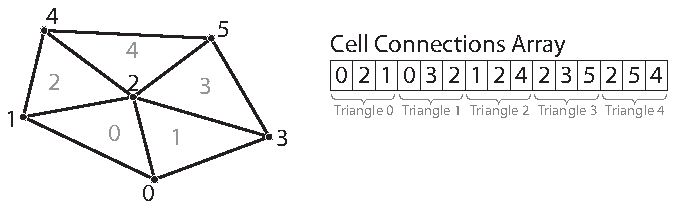
\includegraphics{images/ExplicitCellConnections}
  \caption{An example explicit mesh.}
  \label{fig:ExplicitMesh}
\end{figure}

The \vtkmcont{DataSetBuilderExplicit} class can be used to create data sets
with explicit meshes. \textidentifier{DataSetBuilderExplicit} has several
versions of a method named \textcode{Create}. Generally, these methods take
the shapes, number of indices, and connectivity arrays as well as an array
of point coordinates. These arrays can be given in \textcode{std::vector}
objects, and the data are copied into the \textidentifier{DataSet} created.

The following example creates a mesh like the one shown in
Figure~\ref{fig:ExplicitMesh}.

\vtkmlisting{Creating an explicit mesh with \textidentifier{DataSetBuilderExplicit}.}{CreateExplicitGrid.cxx}

Often it is awkward to build your own arrays and then pass them to
\textidentifier{DataSetBuilderExplicit}. There also exists an alternate
builder class named \vtkmcont{DataSetBuilderExplicitIterative} that allows
you to specify each cell and point one at a time rather than all at once.
This is done by calling one of the versions of \textcode{AddPoint} and one
of the versions of \textcode{AddCell} for each point and cell,
respectively. The next example also builds the mesh shown in
Figure~\ref{fig:ExplicitMesh} except this time using
\textidentifier{DataSetBuilderExplicitIterative}.

\vtkmlisting{Creating an explicit mesh with \textidentifier{DataSetBuilderExplicitIterative}.}{CreateExplicitGridIterative.cxx}

\subsubsection{Add Fields}

In addition to creating the geometric structure of a data set, it is
usually important to add fields to the data. Fields describe numerical data
associated with the topological elements in a cell. They often represent a
physical quantity (such as temperature, mass, or volume fraction) but can
also represent other information (such as indices or classifications).

The easiest way to define fields in a data set is to use the
\vtkmcont{DataSetFieldAdd} class. This class works on
\textidentifier{DataSet}s of any type. It has methods named
\textcode{AddPointField} and \textcode{AddCellField} that define a field
for either points or cells. Every field must have an associated field name.

Both \textcode{AddPointField} and \textcode{AddCellField} are overloaded to
accept arrays of data in different structures. Field arrays can be passed
as standard C arrays or as \textcode{std::vector}s, in which case the data
are copied. Field arrays can also be passed in a
\textidentifier{ArrayHandle}, in which case the data are not copied.

The following (somewhat contrived) example defines fields for a uniform
grid that identify which points and cells are on the boundary of the mesh.

\vtkmlisting{Adding fields to a \textidentifier{DataSet}.}{AddFieldData.cxx}

\index{data~set!Building|)}

\subsection{Cell Sets}
\label{sec:DataSets:CellSets}

\index{cell~set|(}
\index{data~set!cell~set|see{cell~set}}

A cell set determines the topological structure of the data in a data set.
Fundamentally, any cell set is a collection of cells, which typically (but
not always) represent some region in space. 3D cells are made up of points,
edges, and faces. (2D cells have only points and edges, and 1D cells have
only points.) The arrangement of these points, edges, and faces is defined
by the \index{shape}\index{cell~set!shape}\index{cell~shape}\keyterm{shape}
of the cell, which prescribes a specific ordering of each. The basic cell
shapes provided by VTK-m are discussed in detail in
Section~\ref{sec:CellShapeTagsIds} starting on
page~\pageref{sec:CellShapeTagsIds}.

There are multiple ways to express the connections of a cell set, each with
different benefits and restrictions. These different cell set types are
managed by different cell set classes in VTK-m. All VTK-m cell set classes
inherit from \vtkmcont{CellSet}. The two basic types of cell sets are
structured and explicit, and there are several variations of these types.

\subsubsection{Structured Cell Sets}

\index{cell~set!structured|(}
\index{structured~cell~set|(}

A \vtkmcont{CellSetStructured} defines a 1-, 2-, or 3-dimensional grid of
points with lines, quadrilaterals, or hexahedra, respectively, connecting
them. The topology of a \textidentifier{CellSetStructured} is specified by
simply providing the dimensions, which is the number of points in the $i$,
$j$, and $k$ directions of the grid of points. The number of points is
implicitly $i \times j \times k$ and the number of cells is implicitly
$(i-1) \times (j-1) \times (k-1)$ (for 3D grids).
Figure~\ref{fig:CellSetStructured} demonstrates this arrangement.

\begin{figure}
  \centering
  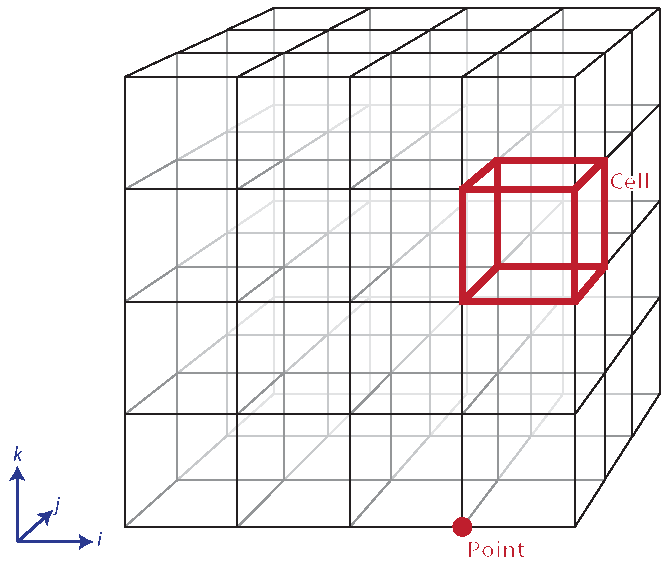
\includegraphics{images/StructuredCellSet}
  \caption{The arrangement of points and cells in a 3D structured grid.}
  \label{fig:CellSetStructured}
\end{figure}

The big advantage of using \vtkmcont{CellSetStructured} to define a cell
set is that it is very space efficient because the entire topology can be
defined by the three integers specifying the dimensions. Also algorithms
can be optimized for \textidentifier{CellSetStructured}'s regular nature.
However, \textidentifier{CellSetStructured}'s strictly regular grid
structure also limits its applicability. A structured cell set can only be
a dense grid of lines, quadrilaterals, or hexahedra. It cannot represent
irregular data well.

Many data models in other software packages, such as the one for VTK, make
a distinction between uniform, rectilinear, and curvilinear grids. VTK-m's
cell sets do not. All three of these grid types are represented by
\textidentifier{CellSetStructured}. This is because in a VTK-m data set the
cell set and the coordinate system are defined independently and used
interchangeably. A structured cell set with uniform point coordinates makes
a uniform grid. A structured cell set with point coordinates defined
irregularly along coordinate axes makes a rectilinear grid. And a
structured cell set with arbitrary point coordinates makes a curvilinear
grid. The point coordinates are defined by the data set's coordinate system,
which is discussed in Section~\ref{sec:DataSets:CoordinateSystems} starting
on page~\pageref{sec:DataSets:CoordinateSystems}.

\index{structured~cell~set|)}
\index{cell~set!structured|)}

\subsubsection{Explicit Cell Sets}

\index{explicit~cell~set|(}
\index{cell~set!explicit|(}

A \vtkmcont{CellSetExplicit} defines an irregular collection of cells. The
cells can be of different types and connected in arbitrary ways. This is
done by explicitly providing for each cell a sequence of points that
defines the cell.

An explicit cell set is defined with a minimum of three arrays. The first
array identifies the shape of each cell. (Cell shapes are discussed in
detail in Section~\ref{sec:CellShapeTagsIds} starting on
page~\pageref{sec:CellShapeTagsIds}.) The second array identifies how many
points are in each cell. The third array has a sequence of point indices
that make up each cell. Figure~\ref{fig:CellSetExplicit} shows a simple
example of an explicit cell set.

\begin{figure}
  \centering
  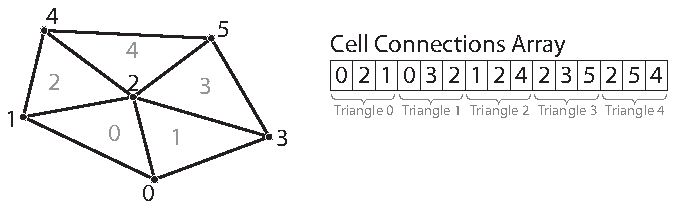
\includegraphics{images/ExplicitCellConnections}
  \caption{Example of cells in a \textidentifier{CellSetExplict} and the
    arrays that define them.}
  \label{fig:CellSetExplicit}
\end{figure}

An explicit cell set may also have other topological arrays such as an
array of offsets of each cell into the connectivity array or an array of
cells incident on each point. Although these arrays can be provided, they
are optional and can be internally derived from the shape, num indices, and
connectivity arrays.

\vtkmcont{ExplicitCellSet} is a powerful representation for a cell set
because it can represent an arbitrary collection of cells. However, because
all connections must be explicitly defined,
\textidentifier{ExplicitCellSet} requires a significant amount of memory to
represent the topology.

\index{cell~set!single~type|(}
\index{explicit~cell~set!single~type|(}
\index{single~type~cell~set|(}

An important specialization of an explicit cell set is
\vtkmcont{CellSetSingleType}. \textidentifier{CellSetSingleType} is an
explicit cell set constrained to contain cells that all have the same shape
and all have the same number of points. So for example if you are creating
a surface that you know will contain only triangles,
\textidentifier{CellSetSingleType} is a good representation for these data.

Using \textidentifier{CellSetSingleType} saves memory because the array of
cell shapes and the array of point counts no longer need to be stored.
\textidentifier{CellSetSingleType} also allows VTK-m to skip some
processing and other storage required for general explicit cell sets.

\index{single~type~cell~set|)}
\index{explicit~cell~set!single~type|)}
\index{cell~set!single~type|)}

\index{cell~set!explicit|)}
\index{explicit~cell~set|)}

\subsubsection{Cell Set Permutations}

\index{permutation~cell~set|(}
\index{cell~set!permutation|(}

A \vtkmcont{CellSetPermutation} rearranges the cells of one cell set to
create another cell set. This restructuring of cells is not done by copying
data to a new structure. Rather, \textidentifier{CellSetPermutation}
establishes a look-up from one cell structure to another. Cells are permuted
on the fly while algorithms are run.

A \textidentifier{CellSetPermutation} is established by providing a mapping
array that for every cell index provides the equivalent cell index in the
cell set being permuted. \textidentifier{CellSetPermutation} is most often
used to mask out cells in a data set so that algorithms will skip over
those cells when running. Note that although
\textidentifier{CellSetPermutation} can mask cells, it cannot mask points.
All points from the original cell set are available in the permuted cell
set regardless of whether they are used.

The following example uses \vtkmcont{CellSetPermutation} with a counting
array to expose every tenth cell. This provides a simple way to subsample a
data set.

\vtkmlisting{Subsampling a data set with \textidentifier{CellSetPermutation}.}{CreateCellSetPermutation.cxx}

\index{cell~set!permutation|)}
\index{permutation~cell~set|)}

\subsubsection{Dynamic Cell Sets}

\index{dynamic~cell~set|(}
\index{cell~set!dynamic|(}

\vtkmcont{DataSet} must hold an arbitrary collection of \vtkmcont{CellSet}
objects, which it cannot do while knowing their types at compile time. To
manage storing \textidentifier{CellSet}s without knowing their types,
\textidentifier{DataSet} actually holds references using
\vtkmcont{DynamicCellSet}.

\textidentifier{DynamicCellSet} is similar in nature to
\textidentifier{DynamicArrayHandle} except that it, of course, holds
\textidentifier{CellSet}s instead of \textidentifier{ArrayHandle}s. The
interface for the two classes is similar, and you should review the
documentation for \textidentifier{DynamicArrayHandle} (in
Section~\ref{sec:DynamicArrayHandle} starting on
page~\pageref{sec:DynamicArrayHandle}) to understand
\textidentifier{DynamicCellSet}.

\vtkmcont{DynamicCellSet} has a method named \textcode{GetCellSet} that
returns a const reference to the held cell set as the abstract
\textidentifier{CellSet} class. This can be used to easily access the
virtual methods in the \textidentifier{CellSet} interface. You can also
create a new instance of a cell set with the same type using the
\textcode{NewInstance} method.

The \textidentifier{DynamicCellSet}\textcode{::IsType()} method can be used
to determine whether the cell set held in the dynamic cell set is of a
given type. If the cell set type is known,
\textidentifier{DynamicCellSet}\textcode{::CastTo()} can be used to safely
downcast the cell set object.

When a typed version of the cell set stored in the
\textidentifier{DynamicCellSet} is needed but the type is not known, which
happens regularly in the internal workings of VTK-m, the
\textcode{CastAndCall} method can be used to make this transition.
\textcode{CastAndCall} works by taking a functor and calls it with the
appropriately cast cell set object.

The \textcode{CastAndCall} method works by attempting to cast to a known
set of types. This set of types used is defined by the macro
\vtkmmacro{VTKM\_DEFAULT\_CELL\_SET\_LIST\_TAG}, which is declared in
\vtkmheader{vtkm/cont}{CellSetListTag.h}. This list can be overridden
globally by defining the \vtkmmacro{VTKM\_DEFAULT\_CELL\_SET\_LIST\_TAG}
macro \emph{before} any VTK-m headers are included.

The set of types used in a \textcode{CastAndCall} can also be changed only
for a particular instance of a dynamic cell set by calling its
\textcode{ResetCellSetList}. This method takes a list of cell types and
returns a new dynamic array handle of a slightly different type that will
use this new list of cells for dynamic casting.

\index{cell~set!dynamic|)}
\index{dynamic~cell~set|}

\subsubsection{Blocks and Assemblies}

Rather than just one cell set, a \vtkmcont{DataSet} can hold multiple cell
sets. This can be used to construct multiblock data structures or
assemblies of parts. Multiple cell sets can also be used to represent
subsets of the data with particular properties such as all cells filled
with a material of a certain type. Or these multiple cells might represent
particular features in the data, such as the set of faces representing a
boundary in the simulation.

\subsubsection{Zero Cell Sets}

It is also possible to construct a \vtkmcont{DataSet} that contains no cell
set objects whatsoever. This can be used to manage data that does not
contain any topological structure. For example, a collection of series that
come from columns in a table could be stored as multiple fields in a data
set with no cell set.

\index{cell~set|)}

\subsection{Fields}
\label{sec:DataSets:Fields}

\index{field|(}
\index{data~set!field|see{field}}

A field on a data set provides a value on every point in space on the mesh.
Fields are often used to describe physical properties such as pressure,
temperature, mass, velocity, and much more. Fields are represented in a
VTK-m data set as an array where each value is associated with a particular
element type of a mesh (such as points or cells). This association of field
values to mesh elements and the structure of the cell set determines how
the field is interpolated throughout the space of the mesh.

Fields are manged by the \vtkmcont{Field} class. \textidentifier{Field}
holds its data with a \textidentifier{DynamicArrayHandle}, which itself is
a container for an \textidentifier{ArrayHandle}. \textidentifier{Field}
also maintains the association and, optionally, the name of a cell set for
which the field is valid.

The data array can be retrieved as a \textidentifier{DynamicArrayHandle}
using the \textcode{GetData} method of \textidentifier{Field}.
\textidentifier{Field} also has a convenience method named
\textcode{GetBounds} that finds the range of values stored in the field
array.

\index{field|}

\subsection{Coordinate Systems}
\label{sec:DataSets:CoordinateSystems}

\index{coordinate~system|(}
\index{data~set!coordinate~system|see{coordinate~system}}

A coordinate system determines the location of a mesh's elements in space.
The spatial location is described by providing a 3D vector at each point
that gives the coordinates there. The point coordinates can then be
interpolated throughout the mesh.

Coordinate systems are managed by the \vtkmcont{CoordinateSystem} class. In
actuality, a coordinate system is just a field with a special meaning, and
so the \textidentifier{CoordinateSystem} class inherits from the
\textidentifier{Field} class. \textidentifier{CoordinateSystem} constrains
the field to be associated with points and typically has 3D floating point
vectors for values.

It is typical for a \textidentifier{DataSet} to have one coordinate system
defined, but it is possible to define multiple coordinate systems. This is
helpful when there are multiple ways to express coordinates. For example,
positions in geographic may be expressed as Cartesian coordinates or as
latitude-longitude coordinates. Both are valid and useful in different
ways.

It is also valid to have a \textidentifier{DataSet} with no coordinate
system. This is useful when the structure is not rooted in physical space.
For example, if the cell set is representing a graph structure, there might
not be any physical space that has meaning for the graph.

\index{coordinate~system|)}

\index{data~set|)}

\section{Timers}
\label{sec:Timers}

\index{timer|(}

It is often the case that you need to measure the time it takes for an
operation to happen. This could be for performing measurements for
algorithm study or it could be to dynamically adjust scheduling.

Performing timing in a multi-threaded environment can be tricky because
operations happen asynchronously. In the VTK-m control environment timing
is simplified because the control environment operates on a single
thread. However, operations invoked in the execution environment may run
asynchronously to operations in the control environment.

To ensure that accurate timings can be made, VTK-m provides a
\vtkmcont{Timer} class that is templated on the device adapter to provide
an accurate measurement of operations that happen on the device. If not
template parameter is provided, the default device adapter is used.

The timing starts when the \textidentifier{Timer} is constructed. The time
elapsed can be retrieved with a call to the \textcode{GetElapsedTime}
method. This method will block until all operations in the execution
environment complete so as to return an accurate time. The timer can be
restarted with a call to the \textcode{Reset} method.

\fix{This example needs to be updated when something interesting can be
  invoked.}

\vtkmlisting{Using \protect\vtkmcont{Timer}.}{Timer.cxx}

\index{timer|)}

\section{Error Handling}
\label{sec:ErrorHandlingControl}

\index{errors|(}

VTK-m uses exceptions to report errors. All exceptions thrown by VTK-m will
be a subclass of \vtkmcont{Error}. For simple error reporting, it is
possible to simply catch a \vtkmcont{Error} and report the error message
string reported by the \textcode{GetMessage} method.

\vtkmlisting{Simple error reporting.}{CatchingErrors.cxx}

There are several subclasses to \vtkmcont{Error}. The specific subclass
gives an indication of the type of error that occured when the exception
was thrown. Catching one of these subclasses may help a program better
recover from errors.
\begin{description}
\item[\vtkmcont{ErrorControlAssert}] \index{assert} \index{errors!assert}
  Thrown when an assertion fails, meaning a VTK-m operation reached an
  unexpected state. The header file \vtkmheader{vtkm/cont}{Assert.h}
  defines a macro named \vtkmmacro{VTKM\_ASSERT\_CONT} that behaves much
  like the POSIX C assert macro except that a
  \textidentifier{ErrorControlAssert} is thrown rather than killing the
  application outright.
\item[\vtkmcont{ErrorControlBadAllocation}] Thrown when there is a problem
  accessing or manipulating memory. Often this is thrown when an allocation
  fails because there is insufficient memory, but other memory access
  errors can cause this to be thrown as well.
\item[\vtkmcont{ErrorControlBadType}] Thrown when VTK-m attempts to perform
  an operation on an object that is of an incompatible type.
\item[\vtkmcont{ErrorControlBadValue}] Thrown when a VTK-m function or
  method encounters an invalid value that inhibits progress.
\item[\vtkmcont{ErrorExecution}] \index{errors!execution~environment} Throw
  when an error is signaled in the execution environment for example when a
  worklet is being executed.
\item[\vtkmcont{ErrorControlInternal}] Thrown when VTK-m detects an
  internal state that should never be reached. This error usually indicates
  a bug in VTK-m or, at best, VTK-m failed to detect an invalid input it
  should have.
\item[\vtkmio{ErrorIO}] Thrown by a reader or writer when a file error is
  encountered.
\end{description}

\index{errors|)}

\index{environment!control|)}
\index{control~environment|)}

